\documentclass[red]{tutorial}
\usepackage[no-math]{fontspec}
\usepackage{xpatch}
	\renewcommand{\ttdefault}{ul9}
	\xpatchcmd{\ttfamily}{\selectfont}{\fontencoding{T1}\selectfont}{}{}
	\DeclareTextCommand{\nobreakspace}{T1}{\leavevmode\nobreak\ }
\usepackage{polyglossia} % English please
	\setdefaultlanguage[variant=us]{english}
%\usepackage[charter,cal=cmcal]{mathdesign} %different font
%\usepackage{avant}
\usepackage{microtype} % Less badboxes

%\usepackage{enumitem}

\usepackage[charter,cal=cmcal]{mathdesign} %different font
%\usepackage{euler}
 
\usepackage{blindtext}
\usepackage{calc, ifthen, xparse, xspace}
\usepackage{makeidx}
\usepackage[hidelinks, urlcolor=blue]{hyperref}   % Internal hyperlinks
\usepackage{mathtools} % replaces amsmath
\usepackage{bbm} %lower case blackboard font
\usepackage{amsthm, bm}
\usepackage{thmtools} % be able to repeat a theorem
\usepackage{thm-restate}
\usepackage{graphicx}
\usepackage{multicol}
\usepackage{fnpct} % fancy footnote spacing
\usepackage{tikz}
\usetikzlibrary{arrows.meta}

\usepackage{pgfplots}
\pgfplotsset{compat=1.18}
%\pgfkeys{/pgf/fpu}

\definecolor{tolBlue}{HTML}{0077BB}
\definecolor{tolCyan}{HTML}{33BBEE}
\definecolor{tolTeal}{HTML}{009988} 
\definecolor{tolOrange}{HTML}{EE7733} 
\definecolor{tolRed}{HTML}{CC3311} 
\definecolor{tolMagenta}{HTML}{EE3377} 
\definecolor{tolGrey}{HTML}{BBBBBB}

 
\newcommand{\xh}{{{\mathbf e}_1}}
\newcommand{\yh}{{{\mathbf e}_2}}
\newcommand{\zh}{{{\mathbf e}_3}}
\newcommand{\R}{\mathbb{R}}
\newcommand{\Z}{\mathbb{Z}}
\newcommand{\N}{\mathbb{N}}
\newcommand{\proj}{\mathrm{proj}}
\newcommand{\Proj}{\mathrm{proj}}
\newcommand{\Perp}{\mathrm{perp}}
\renewcommand{\span}{\mathrm{span}\,}
\newcommand{\Span}{\mathrm{span}\,}
\newcommand{\Img}{\mathrm{img}\,}
\newcommand{\Null}{\mathrm{null}\,}
\newcommand{\Range}{\mathrm{range}\,}
\newcommand{\rref}{\mathrm{rref}}
\newcommand{\rank}{\mathrm{rank}}
\newcommand{\Rank}{\mathrm{rank}}
\newcommand{\nnul}{\mathrm{nullity}}
\newcommand{\mat}[1]{\begin{bmatrix}#1\end{bmatrix}}
\newcommand{\chr}{\mathrm{char}}
\renewcommand{\d}{\mathrm{d}}


\theoremstyle{definition}
\newtheorem{example}{Example}[section]
\newtheorem{defn}{Definition}[section]

%\theoremstyle{theorem}
\newtheorem{thm}{Theorem}[section]

\pgfkeys{/tutorial,
	name={Tutorial 8},
	author={},
	course={MAT 187},
	date={},
	term={},
	title={Linear ODEs}
	}

\begin{document}
	\begin{tutorial}
		\begin{objectives}
	In this tutorial, you will explore separable and first-order linear ODEs.
\end{objectives}

\subsection*{Problems}
\begin{enumerate}
    \begin{minipage}[t]{\linewidth-7cm}

    \item Consider the ODE
\[
    \frac{\mathrm dy}{\mathrm d t} = f(y) = (y-1)^2 (y-2) (y-3)
\]
The graph of $f$ is given on the right.

\textit{You can answer this question based on the equation, the graph, or both!}
\begin{enumerate}
\item Find and classify the equilibrium points of the differential equation. Make sure to justify.
    \vspace{3mm}

\item If $y(t)$ is a solution and $y(0.5)=2.8$, what is $\displaystyle \lim_{t\to\infty} y(t)$? Justify your answer.

\end{enumerate}
\end{minipage}\hfill
\begin{minipage}[t]{6cm}
	\vfil
	\vspace{-6mm}
	\flushright
	\begin{tikzpicture}[line width=1]
	
		\draw [black!20] (-0.5,-1) grid [step=0.5] (4,3);
		\begin{scope}
		\clip (0,-1) rectangle (4,3);
		\draw [smooth,samples=100,domain=0:3.5,tolOrange] plot ({\x},{(\x-1)*(\x-1)*(\x-2)*(\x-3)});
		\end{scope}
	\draw [->] (-0.5,0) -- (4,0) node [right] {$y$};
	\draw [->] (0,-1) -- (0,3) node [above] {$f(y)$};
	\draw (1,0.1) -- (1,-0.1) node [below] {1};
%	\draw (0.1,1) -- (-0.1,1) node [left] {1};
\end{tikzpicture}

\end{minipage}
\item Solve the following initial value problems using separation of variables, and determine over what interval the solution is defined.

\begin{enumerate}
    \item $\frac{\mathrm d y}{\mathrm d x} = 6y^2x$,\qquad $y(1) = \frac{1}{25}$

    \item $\frac{\mathrm d r}{\mathrm d \theta} = \frac{r^2}{\theta},\qquad r(1) = 2 $  

    \item $\frac{\mathrm d y}{\mathrm d t} = e^{-y}(2t-4),\qquad y(5)=0$ 
\end{enumerate}

% \item Consider a pendulum consisting of a massless rod of length $L$ that is connected on one end to an object with mass $m$ and to the ceiling on the other end (via a frictionless hinge). The acceleration due to gravity is $g$. We are interested in understanding the dynamics of the angle $\theta$ between the rod and the negative y-axis.
% \begin{enumerate}
%     \item Determine expressions for the position and velocity of the pendulum with respect to the hinge of the pendulum. Assume the positive x-axis faces rightward, and the positive y-axis faces upward.

%     \item In addition to gravity, there is air resistance that imparts a force in the opposite direction of motion to the pendulum that is proportional to the speed of the mass. This proportionality constant is given by $b$. Write an expression for the air resistance force.

%     \item Write an ODE that models the dynamics of the pendulum.

%     \item Assuming an initial angular position $\theta_0$ and angular velocity $\frac{\mathrm d\theta}{dt}$, write an initial value problem that describes the pendulum.
% \end{enumerate}

\clearpage
\centering 
\includegraphics[scale=1.8]{resources/fish.jpeg}

\raggedright 

\item The graph above depicts the total tons of atlantic cod harvested  year by year from 1850 to the early 2000s on the east coast of Newfoundland. Significant progress in fishing technology led to record-breaking yields in the 1960s. In 1992, the total yield abruptly collapsed to 1\% of historic values, and the industry collapsed completely, destroying a way of life that had sustained the east coast for centuries.
\begin{enumerate}

\item In a few words, why would the harvesting yields decline so rapidly after an increase in harvesting efficiency?


\item You are modelling cod in the ocean with the following setup.
\begin{itemize}
 	\item Let $B(t)$ be the total biomass of cod in the ocean at year $t$ in units of tons.

	\item 
	Let $h(t)$ be the harvesting rate in the year $t$ in units of tons per year.
	\item Let $k$ be the natural growth rate of cod populations. I.e., if there are no other factors, $B(t)=Ae^{kt}$ for some constant $A$. 
	
	\item Let $M$ tons be the maximum cod-carrying capacity of the ocean. That is if there are more than $M$ tons of cod in the ocean, competition for resources will result in unusually high cod death rates.
\end{itemize}

\begin{enumerate}
    \item Write down an ODE that models the cod biomass over time, without harvesting.
    \item Modify the previous ODE so that it includes harvesting.
\end{enumerate}

\item  Assume $h(t)=H$ is constant. Find the equilibrium points of your ODE in terms of $H$, $k$, and $M$. Are they stable or unstable equilibria?

\item Let $k=1$ and $M=100$. How many equilibrium solutions are there if $H=50$? What about if $H=150$?

\item 
Let $k=1$ and $M=100$. For each equilibrium, graph that equilibrium as a function of $H$. Is there a threshold for $H$ where the system changes drastically? What happens to the cod biomass then?

\item Explain in ``real life'' terms what you can learn about cod fishing from your graphs in the previous part.

\end{enumerate}


%\includegraphics[scale=0.7]{tutorials/fish.jpg}
% \item 
% A hungry tiger is hiding in a bush at a position $(L, 0)$, intently watching a gazelle grazing at the origin. To catch the gazelle, the tiger's strategy is to run at a constant speed and towards the gazelle at all times. The gazelle's strategy is to run in the positive $y$ direction at the same speed as the tiger. The equation of motion of the tiger is represented by the differential equation:
	
% 	\[
% 	    \sqrt{1+\left(\frac{dy}{dx}\right)^2} = x\frac{d^2y}{dx^2}
% 	\]
% \begin{enumerate}
% 	    \item Apply the substitution $z=\frac{dy}{dx}$. You should now be able to find $z(x)$ and then $y(x)$, which is the tiger's trajectory.
	    
% 	    \textit{Hint: $\int\sec{\theta}d\theta = \ln\left|\frac{1+\sin\theta}{\cos\theta}\right| + C$.}
%     \item Will the tiger ever catch the gazelle? Justify your answer.

% \end{enumerate}


\end{enumerate}
	\end{tutorial}

	\begin{solutions}
		\begin{enumerate}
\item 
\begin{enumerate}
    \item 
    $y=1$ is semistable,
    $y=2$ is stable,
    $y=3$ is unstable
    
    A visual argument (``If we are just below 1, the derivative is positive, so it's going back to 1'') is nicer than an abstract argument that seems memorized (``If the phase plot crosses from top left to bottom right, it is stable'')

    \item 
    At $y=2.8$, the derivative is negative. The function will decrease. It will continue to do so until $y$ is getting close to 2. The limit will be 2.
\end{enumerate}

\end{enumerate}
	
	\end{solutions}
	\begin{instructions}
		\subsection*{Learning Objectives}
Students need to be able to solve separable and first-order linear ODEs, understand integrating factors, and determine equilibrium points from phase plots.


\subsection*{Notes}
\begin{enumerate}
    \item 
    \item Here are a few standard ODEs for the students to get comfortable applying the solving techniques presented in lecture.
\end{enumerate}


	\end{instructions}

\end{document}
